\chapter[A Quick-Start Guide To Systems-Based Practice]{A Quick-Start Guide To Systems-Based Practice\linebreak Transforming How We Think, Do and Learn}

\openepigraph{%
	An important function of almost every system is to ensure its own perpetuation.
}{Donella H. Meadows}

\marginnote{
	\newthought{Key Message:} You shouldn't have to spend years wandering in the systems thinking 'wilds' like I did. This Chapter outlines three initiatives you can get up and running in Year 1 of your organisation's journey into Systems-Based Practice.
}

\newthought{Increase the effectiveness of your organisation}. There are a lot of things you can do, but we can bundle them into three foci:
\begin{enumerate}
	\item Answer the 'right' questions
	\item Learn together as an organisation
	\item Aim interventions at improving system-outcomes
\end{enumerate}
The first idea shouldn't seem revolutionary, no one wants to waste time focussing on the wrong question. This is all about developing shared-understanding and it can only be done by working 'together'. I know, scary for some. On the plus-side it can be done effectively and efficiently in a virtual environment.
 
The second idea might sound a bit touchy-feeling, but I can assure you this is straight out of the systems dynamics play book and you should be thinking about simulation modelling. Of course it isn't only simulation modelling, but this is such a powerful tool for group learning you avoid it to your organisation's own detriment. However, all sorts of 'modelling' can be invoked -- conceptual, logical, graphical, etc. Your starting place depends where you are as an organisations, but you should be heading towards simulation modelling.

The third idea, if you read the previous two Chapters and didn't just skip to this -- what do I do Chapter, is really the most difficult and will take the most time to implement. This is why you need to get going almost immediately. Don't do what I've done and spend years developing the 'shared-understanding muscles' only to then start really thinking about how you are going to use them to change your system. And yes, system change, is what you are after. This is in essence a 'total quality management' approach to public health practice.

However, you aren't going to get very far if you are unable to bring anyone in your organisation along with you. You need to understand what you are up against.

\section{From Ackoff's Stories to Jackson's Cohesive Approach}

What Ackoff does for 'Mindset' (at least for me), Michael C. Jackson does for 'structurally cohesive approach to problem solving'. In the same way Ackoff deepened my understanding of what it means to use a 'systems perspective' to solve (or rather manage) problems, Jackson sets out a vast, and to me, and an undiscovered landscape of systems thinking with many differing perspectives. Confusion ensues. I found his magnus opus in 2019, and just wow.\cite{Jackson2019} A completely new picture of systems thinking, but dense and heavy with philosophy and social science theory, which I found both revelatory and hard going!

I had already been working on this book for a couple years, when I discovered Jackson's tome. I learned a few things over the next couple of Pandemic-years: 
\begin{enumerate}
	\item As I've said before, I found that I was working with a very restricted view of what systems thinking is or could be (not to worry, I was finding out rapidly that most of my colleagues were in the same boat -- indeed most of them hadn't and still haven't gotten beyond systems dynamics!),
	\item that most of the academics involved in pushing or developing particular systems thinking approaches are more interested in their own world view than they are in helping you, a practitioner, understand how to use it successfully, and
	\item as a consequence their use of language seems to make all of this harder than it ought to be. Their competition for recognition within their respective communities is not helpful to people like you and me, nor is it helping the public sector to adopt this paradigm(s) of thought.
\end{enumerate}

And yet... And yet, despite their best efforts to remain esoteric, which in my experience was exceptionally successful, I was able to understand enough of what Jackson was talking about to understand that you could put a structure around these many divergent efforts to look at the world from a systems perspective. Jackson labels these system-of-systems methodologies or "second-order" methodologies that provide a 'critical' pathway into understanding how all these systems approaches fit together.

\subsection*{Critical Systems Practice -- EPIC}
Jackson's magnus opus and his follow-up practitioner's Guide"\cite{Jackson2024} present Critical Systems Thinking as culmination of the system-of-systems approach. He structures this second-order systems practice approach around a continuous process of critical reflection involving: Explore -- Produce -- Intervene -- Check (Figure~\ref{fig:epic}), which maps out the over-arching methodology of Critical Systems Practice.

\begin{figure}
	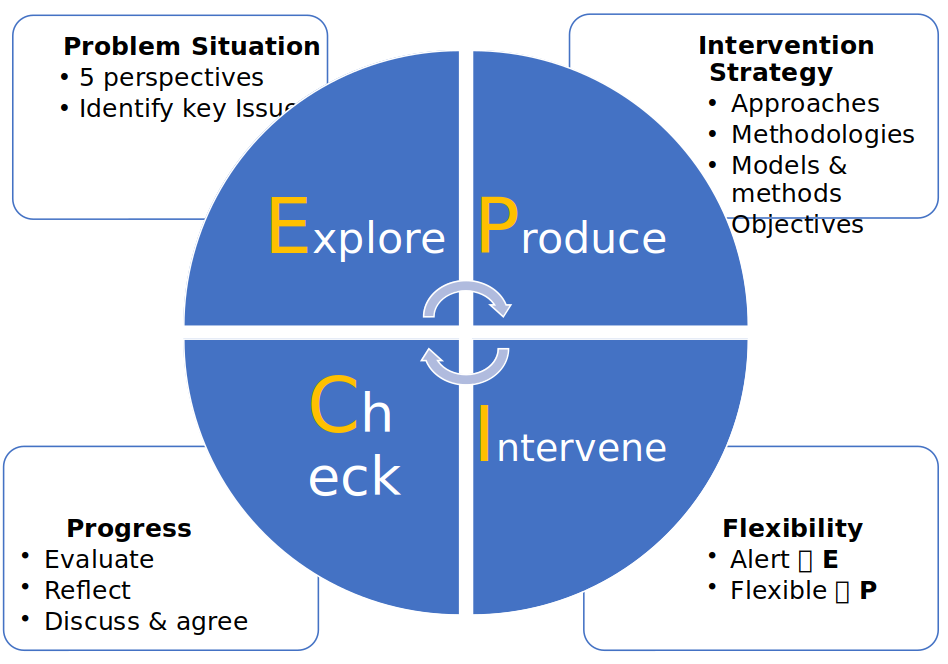
\includegraphics{./figures/epic.png}
	\caption[EPIC -- Critical Systems Practice][6pt]{Critical Systems Practice is implemented through Jackson's EPIC or Explore -- Produce -- Intervene -- Check [Obviously, like many of my diagrams it needs to be redrawn, but it is a good enough placeholder!].}
	\label{fig:epic}
\end{figure}

However, I found his very simple idea (the one he uses to organise the first of these two books), that we can group all methodological approaches into six types or sources of complexity to bring much needed clarity to the systems landscape (Table~\ref{tab:sysapproaches}). Against this classification of complexity, he maps 12 major systems methodologies.

\begin{table}[h]
	\begin{center}
		\footnotesize%
		\begin{tabular}{p{3.5cm} p{6cm}}
			\toprule
			Complexity Challenge & Systems Approaches \\
			\midrule
			Technical Complexity & Operational Research\linebreak  Systems Analysis\linebreak Systems Engineering \\
			Process Complexity & The Vanguard Method \\
			Structural Complexity & System Dynamics \\
			Organisational Complexity & Social-Technical Thinking\linebreak Organisational Cybernetics \\
			People Complexity & Strategic Assumption Surfacing and Testing\linebreak Interactive Planning\linebreak Soft Systems Methodology \\
			Coercive Complexity & Team Syntegrity\linebreak Critical Systems Heuristics \\
			\bottomrule
		\end{tabular}
	\end{center}
	\caption{Matching system problems to approaches, after Jackson 2019}
	\label{tab:sysapproaches}
\end{table}





\section{Get buy-in \& build a coalition for change}

Who is in the market for systems-based public health practice? This is a much different question from who is going to be open to systems thinking ideas -- or almost any new ideas about how to go about something.

Much earlier in my career I read a book on marketing called \emph{Crossing The Chasm}, because I was looking at the challenge of introducing disease spread simulation into public health practice\sidenote{Moore GA. Crossing the Chasm: Marketing and Selling Technology Products to Mainstream Customers. Second Edition. 2004. Capstone. Pages 211.}. I was finding people who were interested. They were everywhere, but they were few in number. Often they were people who were interested in everything, they liked ideas, they liked to play with ideas and to share these ideas. It was always wonderful to find these like minded thinkers!

\emph{Explore}: Problem situation. Examine the situation using five systemic system perspectives: (1) mechanical, (2) interrelationships, (3) organismic, (4) purposeful, and (5) societal/environmental.

\emph{Produce}: Intervention strategy.

\emph{Intervene}: Flexibly.

\emph{Check}: Progress. 

However, as I found out, there is a problem with these like minded thinkers. As Moore's book points out, I'd just learned what innovators are, or at least what some innovators (myself included) are like. We are the first to embrace new ideas, we create pilot projects, we agitate to try x, y and z. Sometimes it catches on sometimes it doesn't.

Moore identified five segments in his "revised technology adoption life cycle". Five segments to conquer -- in public health practice as in anywhere else these are the Innovators, Early adopters, Early majority, Late majority, and Laggards (NEED A MODIFIED FIGURE).

The literature on systems thinking in public health suggests we are now into the early adopters phase. We have more pilots than British Airways (you have no idea how long I've been waiting to use that joke). A select group of people in public health organisations all over the world are putting systems-based public health practice to the test, yet we have not 'crossed the chasm' and we have not moved beyond pilot project tests.

CLIENT CENTRED TRAINING? GREAT PLACE FOR THEIR ENGAGEMENT FIGURE?

\subsection{Never let a crisis go to waste}
Crises, minor panics, tough spots -- these are all natural breaks where for a short period of time people are willing to accept that what they have been doing is no longer working. This happens for a million different reasons. It might not even be declared as such, but they happen and you need to know what they look like in your organisation.

\subsection{Start with your analysts}
There is a clear, but largely unexplored path with your analysts -- if you can seed systems thinking into this group you've created an engine room of problem solving facilitation.

\subsection{Choose your clients carefully}

\subsection{Who should be invited to participate?}

\subsection{Not crisis -- opportunity}
Act when you have their attention. Sometimes it is the only way forward.

\subsection{Picking a good client to get started}


% Place holder Section as I build a readable ToC
\section{Implement new ways of working}
Agile together, humanise the workplace, as part of 'the system'
% Place holder Section as I build a readable ToC
%\section{Doing: Apply shared-understanding to change systems and manage problems}



% Place holder Section as I build a readable ToC
%\section{Learning: Deepen shared-understanding to create organisational learning}
\section{Make it work}
\begin{itemize}
	\item move from expert to facilitator thinking, doing \& learning
	\item replace 'solution' thinking with 'management' thinking
	\item model problems to improve decision-making
\end{itemize}

%\subsection{If you don't know what to expect, how will you know it if you've achieved it?}
The goal is to move public health practice from its 'Hail Mary' approach to setting goals and expectation to a more informed and managed process that improves organisational shared-understanding. There are a number of ways we can do this.
\begin{enumerate}
	\item Logic modelling
	\item Graphical modelling
	\item Simulation modelling
\end{enumerate}

\subsection{System dynamic modelling}

\subsection{Organisational learning -- future directions}




